\section{Requirements}
	\subsection {Unregisterd User Requiremets}
		\subsubsection {System Registration}
			The system needs to enable sign up for new users. This will unlock to the user, after a login, the access to advance features.
			\begin{figure}[!h]
				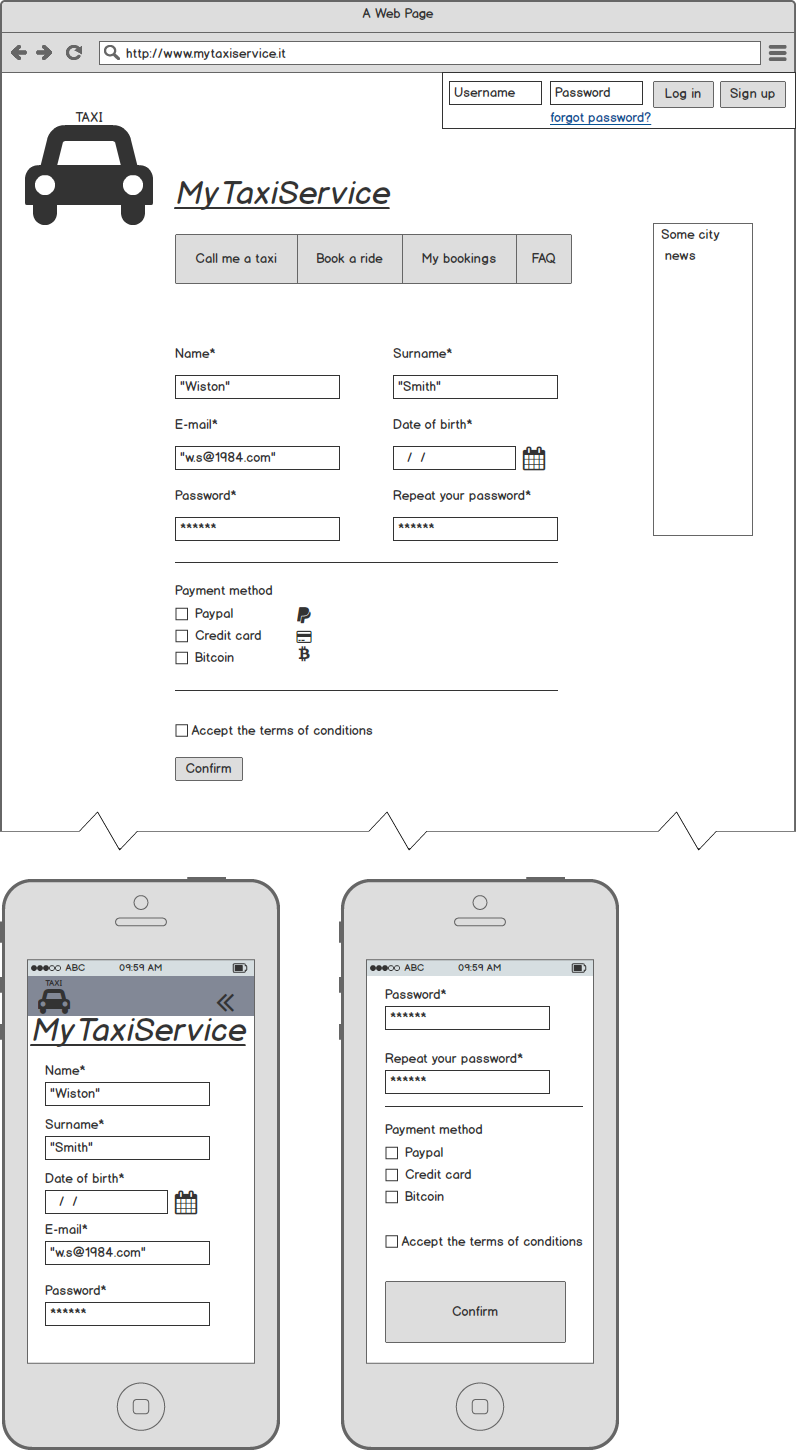
\includegraphics[height=0.7\textheight]{mockup/signup.png}
				\caption{Those mockup show the registration form via web and mobile app.}
			\end{figure}
			\newpage
%\endsubsubsection

		\subsubsection {User Login}
		 	The system must provide an authentication system that enable the access to advanced features.
		\subsubsection {Instant Calls}
			The system must let unregistered user call a taxi immediately.

			When an instant call is made the system will show a popup with a captcha test in order to complete the request.
			\begin{figure}[h!]
				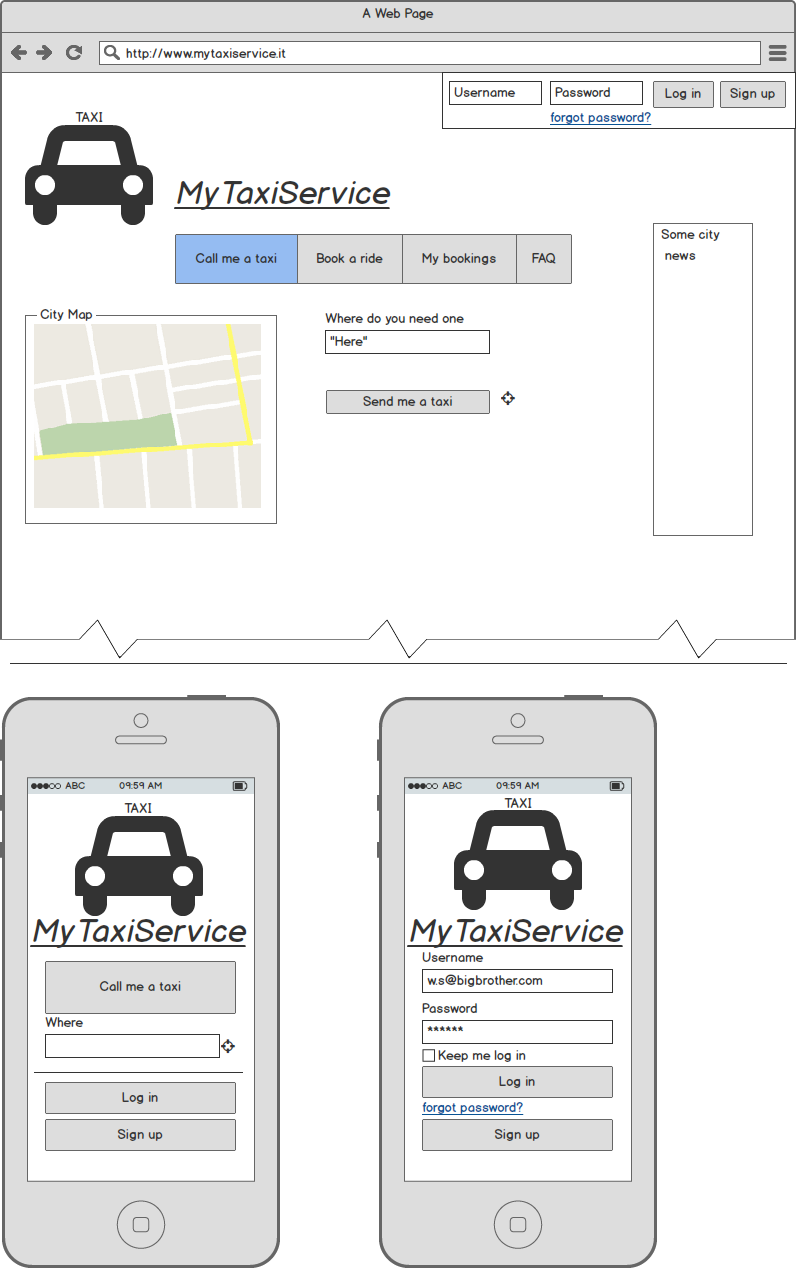
\includegraphics[width=0.6\textwidth]{mockup/home}
				\caption{The home page give the acces to both login and instant call.}
			\end{figure}
			\newpage
	\subsection {Registered User Requirements}
		\subsubsection {User edit information}
			The system must have a profile editing function, where a user can change personal data, such as their address, password, email
			and also add new payment options. On top of that, the system shall log all the rides a user makes into a database.
			\begin{figure}[h!]
				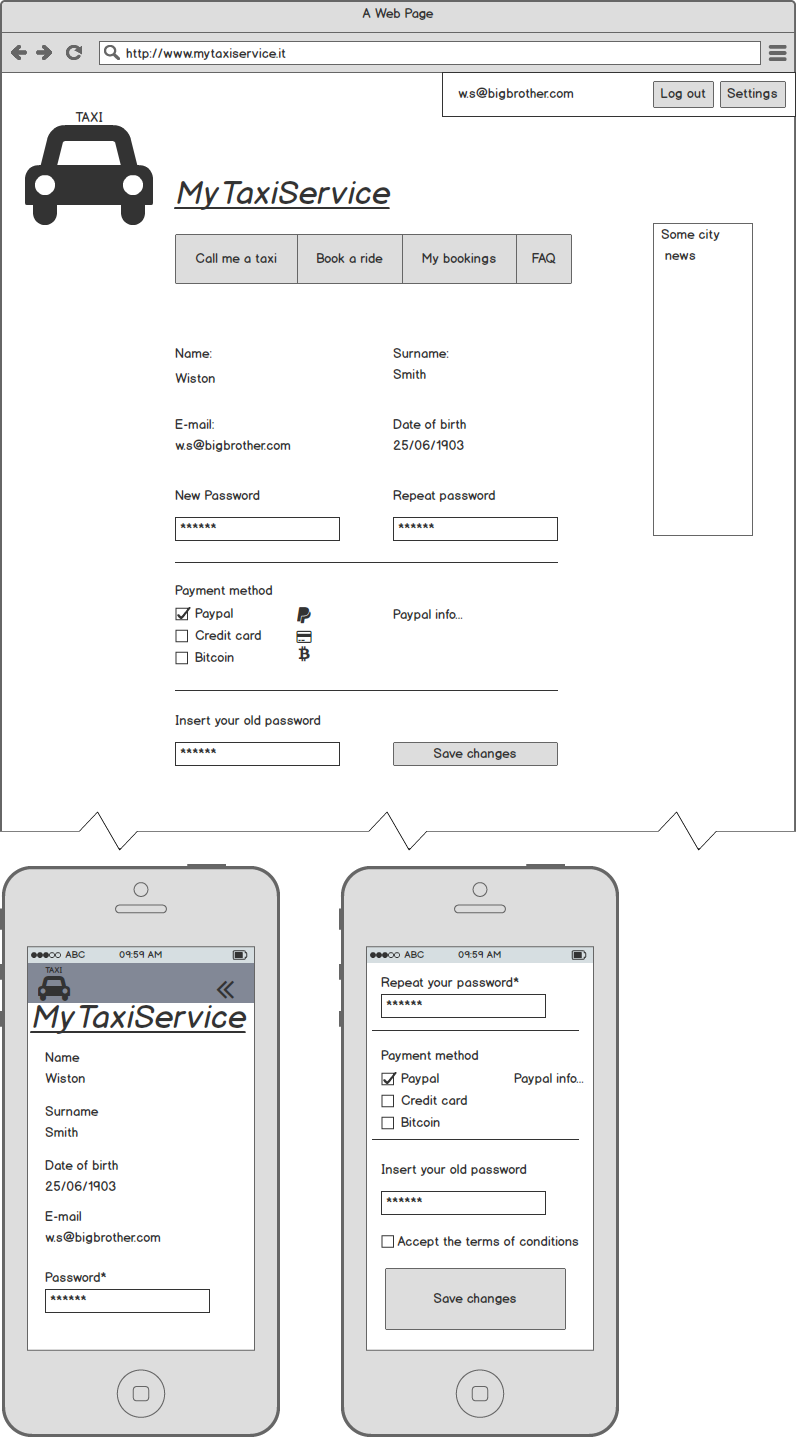
\includegraphics[width=0.6\textwidth]{mockup/edituser.png}
				\caption{Edit form.}
			\end{figure}
			\newpage
		\subsubsection {Instant Calls}
			The system must let registered user call a taxi immediately and give them some advance options.

			When an instant call is made the system will show a popup with a captcha test in order to complete the request.
			\begin{figure}[h!]
				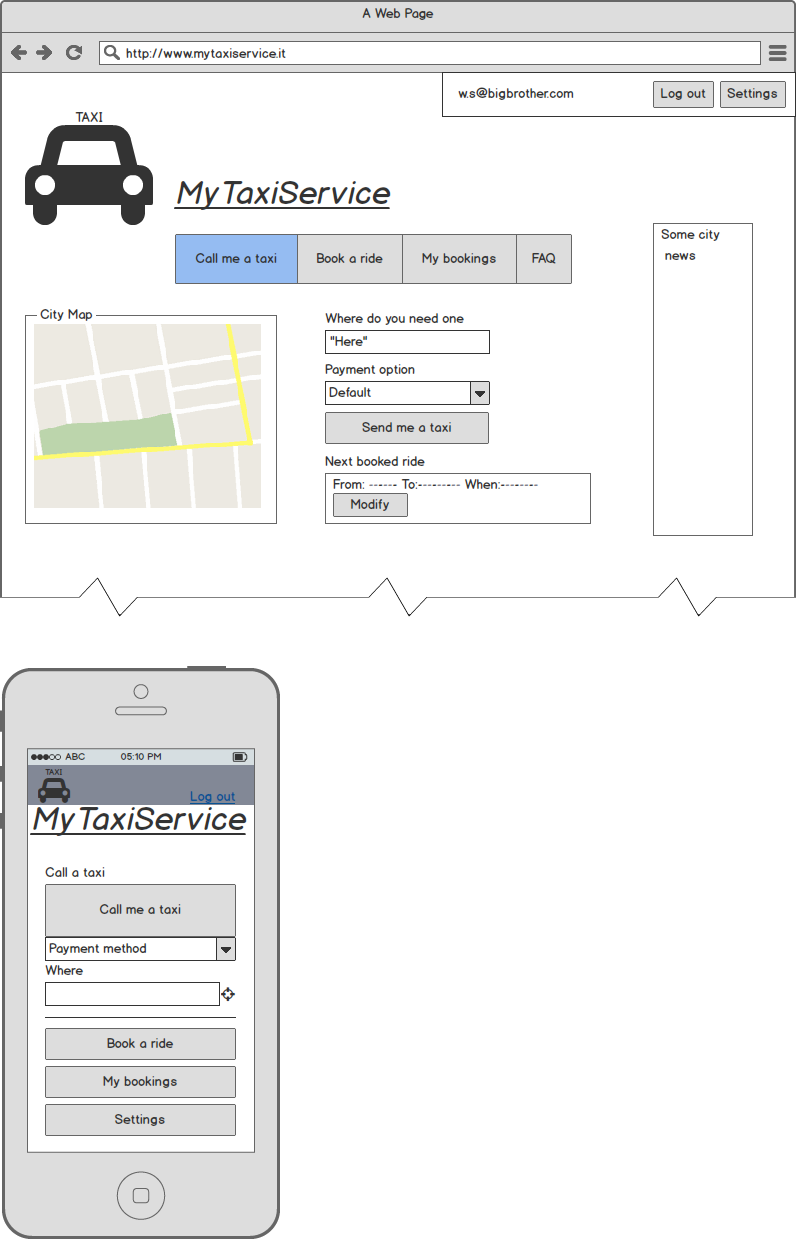
\includegraphics[width=0.6\textwidth]{mockup/homelog}
				\caption{Home page of a logged user.}
			\end{figure}
			\FloatBarrier
			\newpage
		\subsubsection {Booking and Sharing}
			The system must let registered users book a ride for a specific date and time. On top of that, there has to be an option to share
			rides with other people who are booking similar routes. Notifications must be sent when a match is found for shared rides.
			\begin{figure}[!h]
				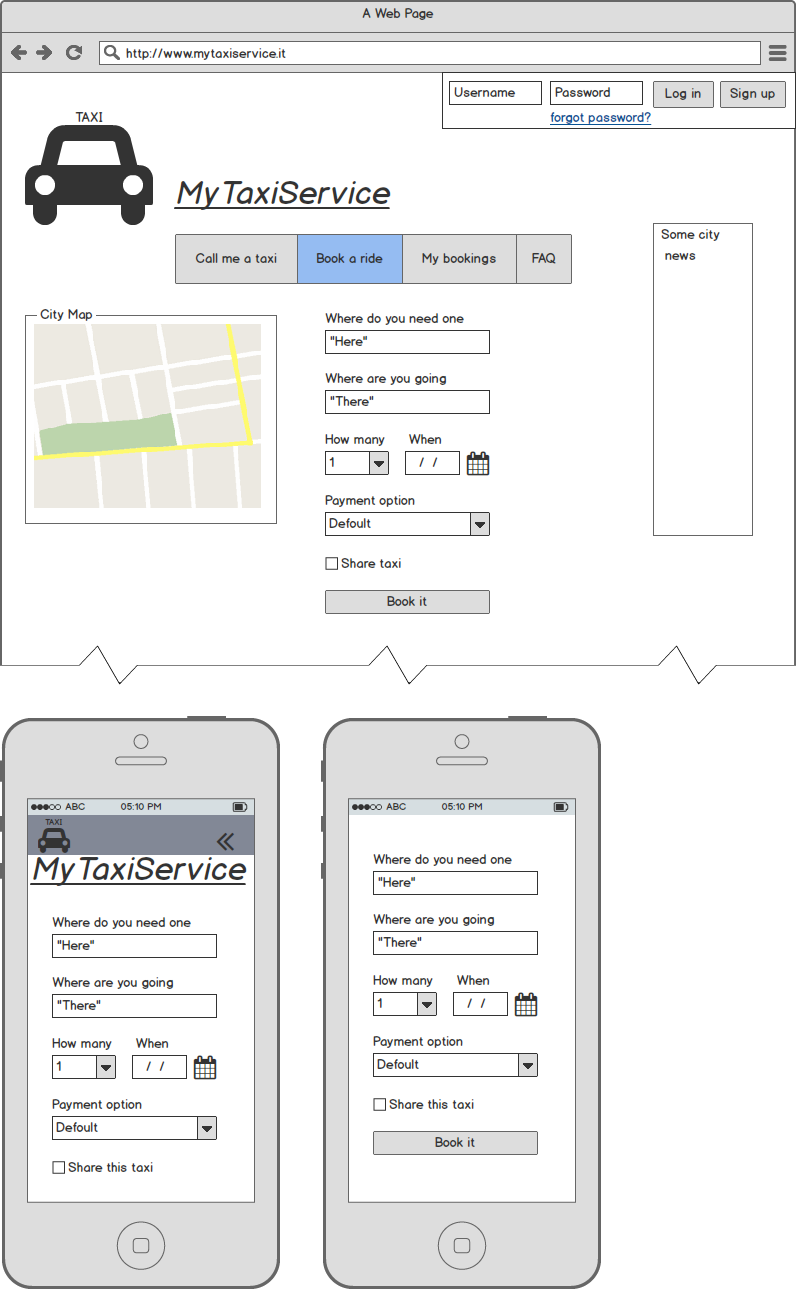
\includegraphics[width=0.6\textwidth]{mockup/bookride}
				\caption{Web and app pages used for book a ride.}
			\end{figure}
			\newpage
		\subsubsection {Booking History}
			The system must let the user to see their booking history and let the acces to the editing of a future ride.
			\begin{figure}[h!]
				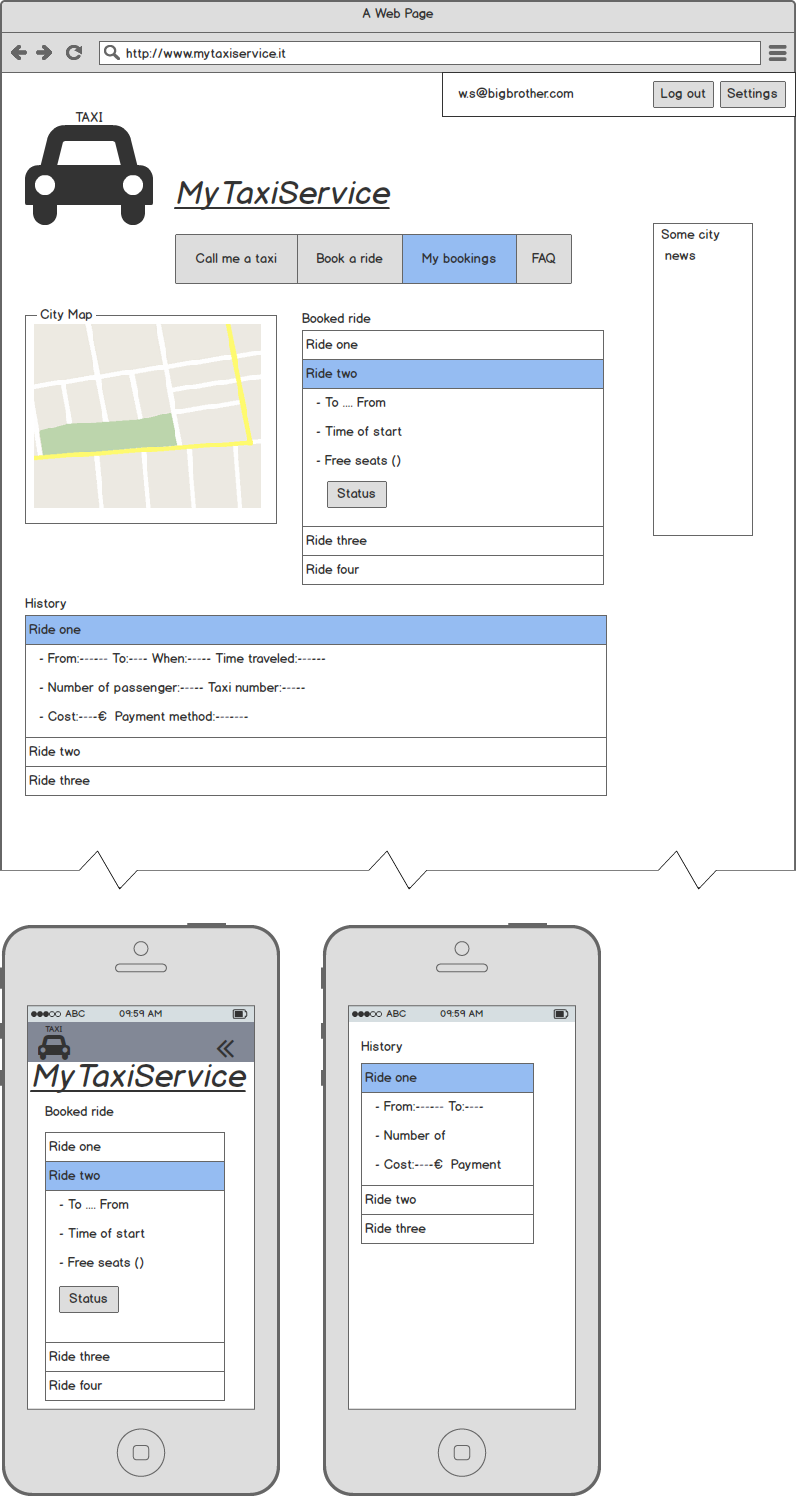
\includegraphics[width=0.6\textwidth]{mockup/history}
				\caption{Booked ride history.}
			\end{figure}
			\newpage
		\subsubsection {Booking Editing}
			The system must let the user to modify or cancel a booked ride (if the ride has not been locked).
			\begin{figure}[h!]
				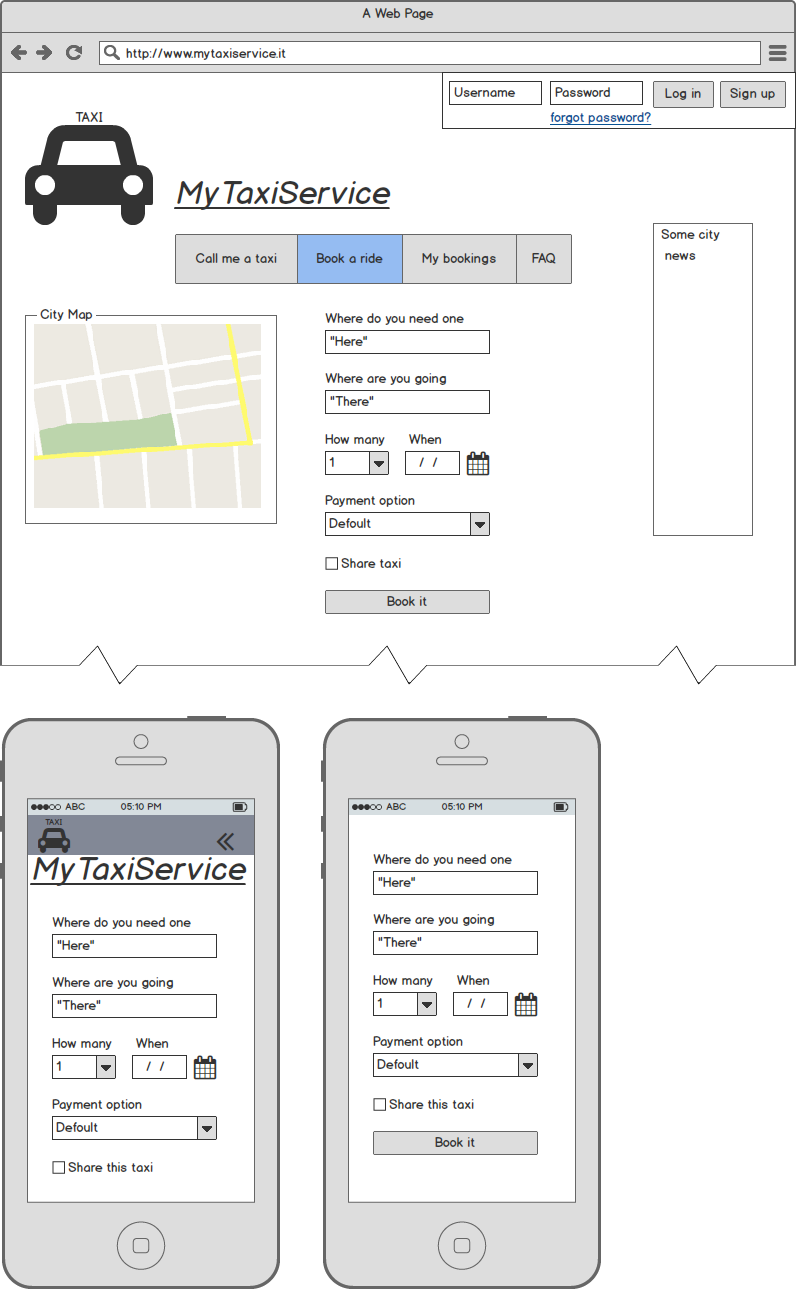
\includegraphics[width=0.6\textwidth]{mockup/bookride}
				\caption{Ride editing form.}
			\end{figure}
			\newpage
	\subsection {Taxi Driver Requirements}
		The worker queue must be handled automatically by the system. This includes building a queue dynamically using a FIFO model.
		\subsubsection {Driver Login}
		 	The system must provide a driver's authentication system that enable the driver to acces his feature.
		 	\begin{figure}[h!]
				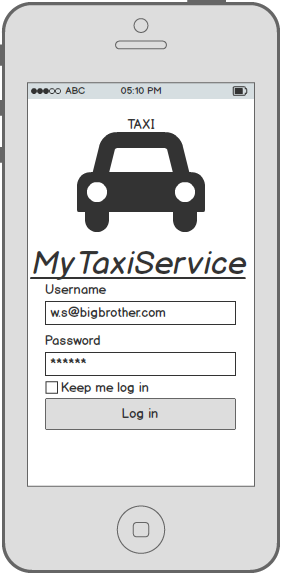
\includegraphics[width=0.6\textwidth, width=3cm]{mockup/driverlogin}
				\caption{Driver's log in interface.}
			\end{figure}
			\newpage
		\subsubsection {Driver Work Settings}
		 	The system must provide the driver the acces to his working condition.
		 	\begin{figure}[h!]
				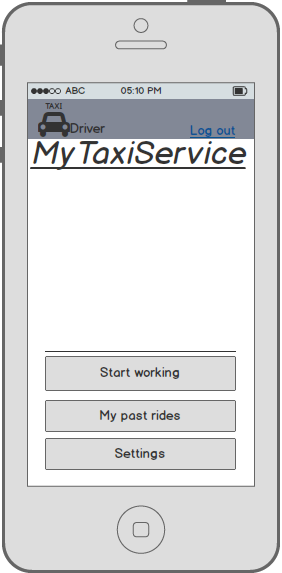
\includegraphics[width=0.6\textwidth, width=3cm]{mockup/appdriverlogged}
				\caption{Driver's home page.}
			\end{figure}
			\newpage
		\subsubsection {Driver Ride Acceptance}
			The system must provide the driver to accept or refuse a ride.
		 	\begin{figure}[h!]
				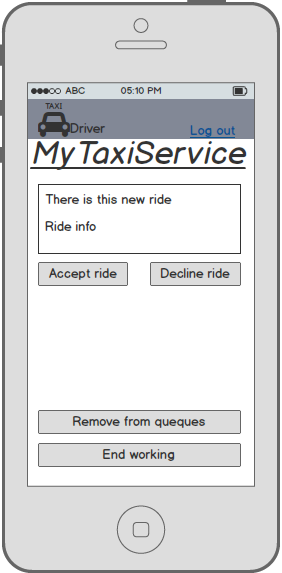
\includegraphics[width=0.6\textwidth, width=3cm]{mockup/appdrivernew}
				\caption{Driver's ride information page.}
			\end{figure}
			\newpage
		\subsubsection {Driver Ride Settings}
			The system must provide the driver information on the ride and a command to end it, and a function that automatically reinserts into the queue.
		 	\begin{figure}[h!]
				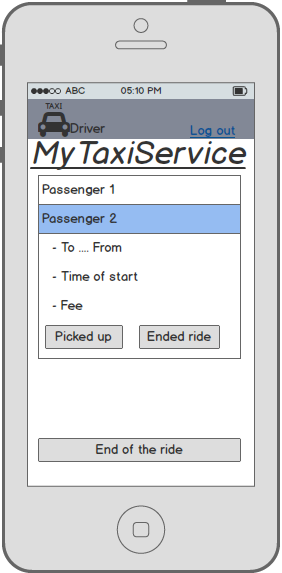
\includegraphics[width=0.6\textwidth, width=3cm]{mockup/appdriveron}
				\caption{Driver's ride information page.}
			\end{figure}
			\newpage

%\endsubsection
\subsection{Functional Requirements}
	After having stated the effective requirements for the system, we can start listing what a user can do.
		\begin{description}
		\item[Unregistered user/Guest] \hfill
			\begin{itemize}
				\item Sign up
				\item Log in
				\item Instant call
			\end{itemize}
		\item[Registered User] \hfill
			\begin{itemize}
				\item Instant call
				\item Change user data, including payment options
				\item View ride history
				\item Advance booking(with sharing options)
				\item Booking modifications
				\item View booking status(including sharing status)
				\item Logout
			\end{itemize}
		\item[Taxi Driver] \hfill
			\begin{itemize}
				\item Set work status
				\item Start a ride
				\item Accept or refuse a ride
				\item Notify end of ride
				\item Logout
			\end{itemize}
		\end{description}
%\endsubsection
\newpage
\subsection{Logical Database Requirements}
	A database should be put in place server-side to handle credential storage, ride booking and ride history. The database responsible for ride history
	shall include where the each ride started and ended, the taxi carrying the passengers and the corresponding driver, and the user/s that made use of the
	taxi(multiple users, up to 4, in case of a shared ride). Note that rides made by unregistered users should also be logged, so drivers may view their own history.
%\endsubsection
\subsection {Non Functional Requirements}
 	\subsubsection{Performance Requirements}
 		The system should be fast in order to garantee a good service to the final user. We  assume that our system response to the users need is close to zero.
	\subsubsection {Design Constraint}
		The main system will be developed using Java EE, we also have to develope two mobile applications in
		Objective-C and Java.
	\subsubsection {System Avaibility}
		The service will be accesible online both via web and mobile-app. To achieve this we will use a Cloud Virtual Server provider. This will guarantee more scalability
		for the system and can also reduce the cost that we would have with dedicated server. On top of that we can maintain high level performances even in busy days
%\endsubsection
\subsection {Security}
	My Taxi Service implements a login authentication in order to protect user's sensible informations. Password must be 8 character long and must contain both letters
	and numbers. Password will be encrypted and stored in the database with all user's data.

	We guarantee that the user can't acces to other user sensible information.

	At sign up the user will recive an email with a confirmation link to enable the acces to the advanced feature of our system.

	We also implement a capcha control when you make an instant call, in order to prevent missclick or botnet attack.
%\endsubsection